% Generado por a_pdf.py desde reporte.md -- no editar a mano
\documentclass[11pt,a4paper]{article}
\usepackage[utf8]{inputenc}
\usepackage[T1]{fontenc}
\usepackage[spanish,mexico]{babel}
\usepackage{graphicx}
\usepackage[margin=2.5cm]{geometry}
\usepackage{amsmath}
\usepackage{booktabs}
\usepackage{tabularx}
\usepackage{array}
\usepackage{fvextra}
\usepackage{float}
\usepackage{setspace}
\usepackage{parskip}
\usepackage{fancyhdr}
\usepackage{textcomp}
\usepackage[hidelinks]{hyperref}

\onehalfspacing
\setlength{\parskip}{6pt}
\sloppy
\setlength{\emergencystretch}{3em}
\setlength{\headheight}{40pt}
\pagestyle{fancy}
\fancyhf{}
\fancyhead[L]{\includegraphics[width=1cm]{/home/yovick/repos/UAZ-IEI/Assets/UIE.png}}
\fancyhead[R]{\small Comunicaciones Inalámbricas}
\fancyfoot[C]{\thepage}
\renewcommand{\headrulewidth}{0.4pt}

\begin{document}

% ---------------------------- PORTADA -----------------------
\begin{titlepage}
  \thispagestyle{empty}
  \begin{center}
    \vspace*{1cm}
    \includegraphics[width=4.5cm]{/home/yovick/repos/UAZ-IEI/Assets/uaz.png}
    \vspace{0.8cm}

    {\large Universidad Autónoma de Zacatecas}\\[4pt]
    {\large Unidad Académica de Ingeniería Eléctrica}\\[4pt]
    {\normalsize Ingeniería Electrónica Industrial con especialidad en Telecomunicaciones}

    \vspace{1.8cm}
    {\LARGE\bfseries Práctica 5}\\[10pt]
    {\Large\bfseries Caracterización experimental del efecto Doppler y tiempo de coherencia}
  \end{center}

  \vspace{2.2cm}
  \begin{center}
    \begin{tabular}{rl}
      \textbf{Materia:} & Comunicaciones Inalámbricas\\
      \textbf{Docente:} & Dr. Víktor Iván Rodríguez Abdalá\\
      \textbf{Alumno:}  & Arnold Yovick Ríos Zaldívar\\
      \textbf{Fecha:}   & Octubre de 2026\\
    \end{tabular}
  \end{center}
  \vfill
\end{titlepage}

\textbf{Equipo:} RTL-SDR (\texttt{RTL2832U} + tuner \texttt{R820T}), antena telescópica, fuente CW en 433.9 MHz

\textbf{Script:} \texttt{practica5.py} (Python; el análisis MATLAB del manual se implementa con NumPy/SciPy)

\section{Objetivo}

Analizar experimentalmente el efecto Doppler en un canal inalámbrico móvil a partir de la envolvente de una fuente de onda continua (CW) recibida en tres escenarios de movilidad del receptor (estático, caminando lento y caminando rápido). Se busca:

\begin{itemize}
  \item Observar la variación temporal de la envolvente del canal.
  \item Obtener el espectro Doppler de la envolvente y del canal.
  \item Estimar la frecuencia Doppler máxima $f_D$.
  \item Calcular el tiempo de coherencia $T_c \approx 0.423/f_D$ y relacionarlo con la velocidad.
\end{itemize}

\section{Fundamento teórico}

\subsection{Efecto Doppler}

Cuando el receptor se mueve respecto al transmisor con velocidad relativa $v$, la frecuencia observada difiere de la transmitida:

\[
f = f_c\left(1 \pm \frac{v}{c}\right) \quad\Rightarrow\quad \Delta f = \frac{v}{\lambda}\cos\theta
\]

donde $\lambda = c/f_c$ es la longitud de onda y $\theta$ es el ángulo entre la dirección de movimiento y la dirección de llegada de la onda. La \textbf{frecuencia Doppler máxima} ocurre para $\theta = 0$:

\[
f_D = \frac{v}{\lambda} = \frac{v\,f_c}{c}
\]

Para 433.9 MHz, $\lambda = 0.691$ m, de modo que $f_D \approx 1.45\,\mathrm{Hz}$ por cada m/s de velocidad. En un canal con multitrayectoria, cada réplica llega con un ángulo (y por tanto un desplazamiento Doppler) distinto: la superposición ensancha el espectro alrededor de $f_c$ y hace que la amplitud y la fase de la señal varíen en el tiempo (\textbf{desvanecimiento selectivo en el tiempo}).

\subsection{Espectro Doppler}

Para dispersión isotrópica (modelo de Clarke/Jakes) el espectro de potencia del canal en banda base tiene forma de "U" con soporte $[-f_D, f_D]$ y densidades infinitas en los bordes. La dispersión Doppler (ancho del espectro) es del orden de $2f_D$ entre primer y último rayo.

La \textbf{envolvente} $r(t) = |x(t)|$ de una señal CW desvanecida fluctúa con la misma escala de tiempo. Su espectro de fluctuaciones (con la media removida) es aproximadamente la \textbf{autoconvolución} del espectro Doppler del canal, por lo que se extiende hasta $\approx 2f_D$ y resulta $\approx\sqrt{2}$ más ancha que el espectro del canal complejo.

\subsection{Tiempo de coherencia}

El tiempo de coherencia $T_c$ es el intervalo durante el cual la respuesta del canal puede considerarse aproximadamente constante (la autocorrelación temporal se mantiene por encima de un umbral, típicamente 0.5). Se aproxima mediante

\[
T_c \approx \frac{0.423}{f_D}
\]

de modo que $T_c$ es inversamente proporcional a la velocidad: a mayor movilidad, canal más rápido y menor $T_c$. Valores de referencia para 433.9 MHz:

\begin{tabularx}{\linewidth}{@{}*{5}{>{\raggedright\arraybackslash}X}@{}}
\toprule
Escenario & $f_D$ (Hz) & $v = f_D\lambda$ (m/s) & $v$ (km/h) & $T_c$ teórico (s) \\
\midrule
Estático (leve balanceo) & 0.2 & 0.14 & 0.5 & 2.115 \\
Caminando lento & 3.0 & 2.07 & 7.5 & 0.141 \\
Caminando rápido & 12.0 & 8.29 & 29.9 & 0.035 \\
\bottomrule
\end{tabularx}

\begin{quote}
El mismo $f_D$ corresponde a velocidades menores si se sube la frecuencia portadora (en 915 MHz, como en el manual, $\lambda = 0.328$ m: $f_D = 3$ Hz equivale a 0.98 m/s y 12 Hz a 3.9 m/s).
\end{quote}

\section{Desarrollo experimental}

\subsection{Configuración del receptor}

\begin{tabularx}{\linewidth}{@{}*{2}{>{\raggedright\arraybackslash}X}@{}}
\toprule
Parámetro & Valor \\
\midrule
Chip / tuner & RTL2832U / R820T \\
Frecuencia central & \textbf{433.9 MHz} (banda ISM; el manual propone 915 MHz) \\
Sample rate & 240 kHz (como el manual) \\
Muestras por escenario (ventana móvil \texttt{--dur}) & $n = \lfloor 5\,\mathrm{s}\cdot 240\,\mathrm{kHz}\rfloor = 1\,200\,000$ \\
Filtro IF del tuner & 600 kHz (\texttt{--bw}) \\
Ganancia & \texttt{auto}: la mayor que no recorta el ADC (\texttt{--gain} permite fijarla) \\
Antena & telescópica conectada al RX \\
Captura & asíncrona, sin pérdida de muestras (\texttt{vivo.Fuente}) \\
\bottomrule
\end{tabularx}

\subsection{Escenarios}

\begin{tabularx}{\linewidth}{@{}*{3}{>{\raggedright\arraybackslash}X}@{}}
\toprule
Escenario & $f_D$ nominal & Instrucción al usuario \\
\midrule
\texttt{estatico} & 0.2 Hz & Permanecer quieto con el receptor en la mano \\
\texttt{lento} & 3 Hz & Caminar despacio y sostener el paso durante los 5 s de captura \\
\texttt{rapido} & 12 Hz & Caminar rápido y sostener el paso durante los 5 s de captura \\
\bottomrule
\end{tabularx}

El transmisor CW permanece fijo; solo se mueve el receptor. El modo real abre la ventana en vivo: el escenario se elige con \texttt{1}, \texttt{2} o \texttt{3} y la medición se fija con \texttt{ESPACIO} sobre la ventana móvil de \texttt{--dur} segundos. El modo \texttt{--sim} genera los mismos escenarios sin dongle y \texttt{--selftest} verifica el estimador.

\subsection{Procedimiento}

\begin{enumerate}
  \item \texttt{python3 practica5.py} (real) o \texttt{python3 practica5.py --sim} (sintético).
  \item Por escenario se acumula la ventana móvil de \texttt{--dur} segundos, se obtiene la envolvente $r=|x|$ y su PSD con Welch.
  \item Se estima $f_D$ y se calcula $T_c = 0.423/f_D$.
  \item La tecla \texttt{s} guarda \texttt{figs/envolventes.png}, \texttt{figs/doppler.png} y \texttt{datos/resultados.json}.
\end{enumerate}

\textbf{Simulación (\texttt{--sim}).} Cada escenario se genera con \texttt{vivo.ruido\_plano}, un desvanecimiento de espectro Doppler plano con ancho \texttt{fd} (0.2, 3 y 12 Hz nominales) sintetizado a \texttt{max(20\textperiodcentered{}fd, 1 kHz)} y llevado a la tasa del receptor conservando el estado entre bloques, multiplicado por una portadora compleja constante (equivalente al IQ de una fuente CW). Se usa una semilla fija para que los resultados sean reproducibles.

\section{Código}

El script completo está en \texttt{practica5.py}. Fragmentos esenciales:

\begin{Verbatim}[breaklines=true,breakanywhere=true,fontsize=\small]
# Simulación: envolvente de espectro Doppler plano (vivo.ruido_plano)
gen = vivo.ruido_plano(rate, fd=FD_ESC[NOMBRES[self.sel]][0])
x = gen(n) * np.exp(1j*np.pi/4)                         # portadora CW constante

# PSD de Welch centrada (método del manual para el IQ)
f_man, P_man = _psd(x, fs, 4096, 2048, 4096)             # welch(x, fs, 4096, 2048, 4096)

# Espectro Doppler de la envolvente (decimada a 240 Hz para resolver pocos Hz)
L = max(1, int(round(fs / FS_ENV)))
xd = resample_poly(x, 1, L)
r = np.abs(xd)
f_env, P_env = _psd(r - r.mean(), fs/L, 1024, nfft=8192)

# Estimación: ancho RMS y corrección por autoconvolución
sigma = np.sqrt((f_env**2 * P_env).sum() / P_env.sum())
fD = np.sqrt(1.5) * sigma
Tc = 0.423 / fD
\end{Verbatim}

La PSD del IQ a la tasa completa (\texttt{welch(x, fs, 4096, 2048, 4096, return\_onesided=False)}) se conserva por ser el método del manual, pero su resolución es $f_s/4096 = 58.6$ Hz: no puede resolver $f_D$ de pocos Hz. Por eso el espectro Doppler se calcula sobre la envolvente decimada a 240 Hz (anti-alias con \texttt{resample\_poly}), donde la resolución es de 0.03 Hz.

\section{Resultados}

\begin{quote}
\textbf{Los resultados de esta sección corresponden a una verificación por simulación (\texttt{--sim}, semilla fija) y NO a la corrida real.} Se muestran para validar el procesamiento sin ocupar el dongle; deben reemplazarse con los datos de la corrida real con el transmisor CW y el receptor en movimiento.
\end{quote}

\subsection{Mediciones}

\begin{tabularx}{\linewidth}{@{}*{6}{>{\raggedright\arraybackslash}X}@{}}
\toprule
Escenario & $f_D$ teórico (Hz) & $f_D$ estimado (Hz) & $T_c$ teórico (s) & $T_c$ medido (s) & Ancho RMS $\sigma$ (Hz) \\
\midrule
Estático & 0.2 & 1.04 & 2.115 & 0.407 & 0.85 \\
Lento & 3.0 & 3.06 & 0.141 & 0.138 & 2.50 \\
Rápido & 12.0 & 12.70 & 0.035 & 0.033 & 10.37 \\
\bottomrule
\end{tabularx}

Salida de consola de la corrida:

\begin{tabularx}{\linewidth}{@{}*{4}{>{\raggedright\arraybackslash}X}@{}}
\toprule
Escenario & fD (Hz) & Tc (s) & Ancho PSD (Hz) \\
\midrule
Estatico & 1.04 & 0.407 & 0.85 \\
Lento & 3.06 & 0.138 & 2.50 \\
Rapido & 12.70 & 0.033 & 10.37 \\
\bottomrule
\end{tabularx}

\texttt{--selftest} (escenario lento, exige $1.5 < f_D < 6$ Hz):

\begin{Verbatim}[breaklines=true,breakanywhere=true,fontsize=\small]
practica5 selftest OK
\end{Verbatim}

\subsection{Variación temporal de la envolvente}

\begin{center}
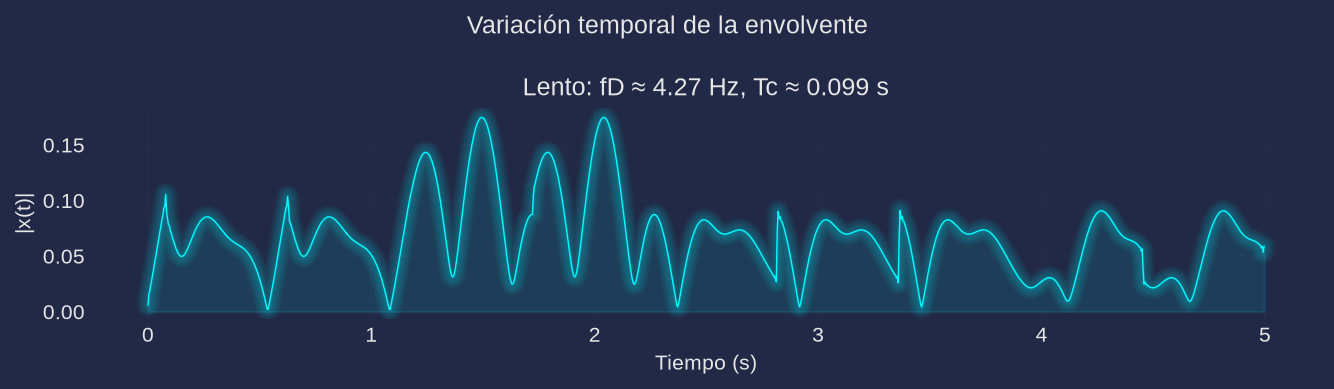
\includegraphics[width=0.9\linewidth]{figs/envolventes.png}\\[2pt]
{\small Envolventes de los tres escenarios}
\end{center}

La envolvente estática varía lentamente (unos pocos desvanecimientos en 5 s); al caminar lento aparecen mínimos profundos separados por décimas de segundo, y al caminar rápido la amplitud cambia varias veces por segundo. El ritmo de fluctuación crece con la velocidad, como predice $f_D = v/\lambda$.

\subsection{Espectro Doppler}

\begin{center}
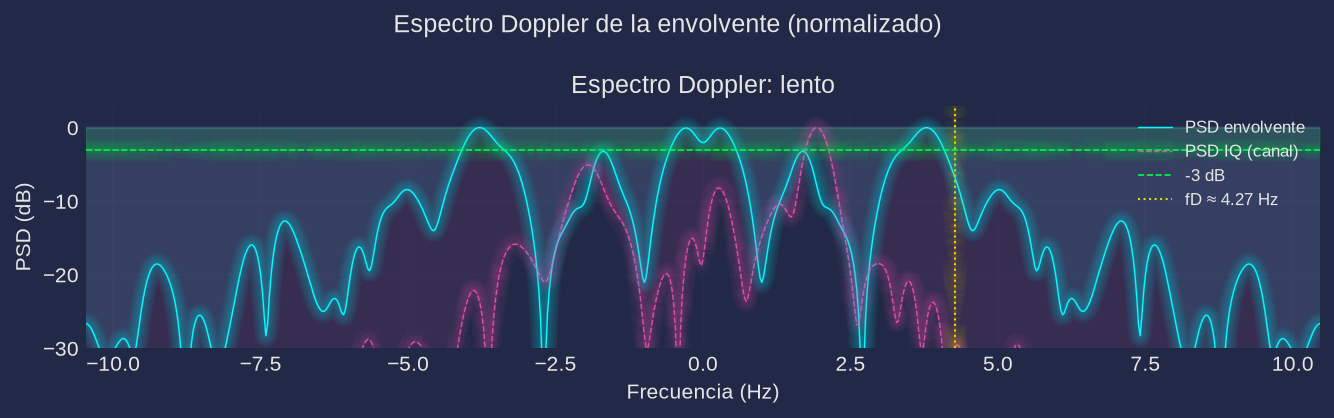
\includegraphics[width=0.9\linewidth]{figs/doppler.png}\\[2pt]
{\small Espectro Doppler de los tres escenarios}
\end{center}

En cada panel se muestra la PSD normalizada de la envolvente (línea llena, media removida) y la PSD del canal IQ (discontinua), con la línea de $-$3 dB y el valor estimado de $f_D$. El ensanchamiento del espectro es evidente: la anchura RMS pasa de 0.85 Hz (estático) a 2.50 Hz (lento) y 10.37 Hz (rápido), aproximadamente proporcional a $f_D$. La PSD de la envolvente es más ancha que la del canal porque es su autoconvolución.

\subsection{Criterio de estimación}

El cruce puntual de $-$3 dB sobre la PSD de la envolvente resultó poco confiable con registros de 5 s (pocos ciclos de desvanecimiento y alto rizo del periodograma: valores de 0.50, 1.31 y 1.52 Hz que no escalan con la velocidad). Se adoptó un \textbf{ancho RMS}: para un espectro Doppler plano de ancho $f_D$, la PSD de las fluctuaciones de la envolvente es su autoconvolución (triangular) y su varianza es $\sigma^2 = 2f_D^2/3$; por lo tanto

\[
f_D = \sqrt{\tfrac{3}{2}}\,\sigma
\]

El estimador es lineal con la velocidad (3.06 y 12.70 Hz frente a 3 y 12 Hz nominales) y el cruce crudo de $-$3 dB se conserva en \texttt{datos/resultados.json} como \texttt{ancho\_3dB\_Hz}.

En el escenario estático el valor medido (1.04 Hz) no es el $f_D$ real (0.2 Hz) sino el \textbf{piso de resolución del método}: con 5 s de registro solo se observa 1 ciclo de un proceso de 0.2 Hz, y el generador sintético (sintetizado a \texttt{max(20\textperiodcentered{}fd, 1 kHz)}) tampoco resuelve esa frecuencia. Para medirlo habría que capturar varias decenas de segundos.

\section{Análisis de resultados}

\begin{enumerate}
  \item \textbf{Efecto de la velocidad sobre el espectro.} El ensanchamiento Doppler crece de forma aproximadamente proporcional a la velocidad: $\sigma = 0.85 \to 2.50 \to 10.37$ Hz. Al pasar de lento a rápido la anchura se multiplica por 4.15, consistente con el factor 4 entre $f_D = 3$ y 12 Hz. El espectro de la envolvente se extiende hasta $\approx 2f_D$ ($\approx$24 Hz en el escenario rápido), lo que se aprecia en los paneles al comparar la PSD de la envolvente con la del canal.
  \item \textbf{Relación $f_D$--$T_c$.} Los valores medidos cumplen $T_c \approx 0.423/f_D$ ($T_c = 0.138$ s con $f_D = 3.06$ Hz y $T_c = 0.033$ s con $f_D = 12.70$ Hz). Al duplicar la velocidad se duplica $f_D$ y se reduce $T_c$ a la mitad: el canal cambia el doble de rápido.
  \item \textbf{Implicaciones.} Un $T_c$ pequeño limita el tiempo durante el cual una estimación de canal sigue siendo válida: con $T_c \approx 0.14$ s (lento) los pilotos deben repetirse al menos cada \textasciitilde{}0.14 s; con $T_c \approx 33$ ms (rápido) se necesitan estimadores y ecualizadores que sigan el canal en esa escala. Si la duración de símbolo o de bloque supera $T_c$, aparecen errores de estimación, pérdida de ortogonalidad entre subportadoras (ICI en OFDM) y degradación de la BER. En el extremo opuesto, el desvanecimiento rápido también se explota con diversidad temporal e intercalado.
  \item \textbf{Dependencia con la frecuencia y el ángulo.} $f_D = v\cos\theta/\lambda$: a mayor portadora, mayor $f_D$ para la misma velocidad (en 915 MHz las velocidades equivalentes son \textasciitilde{}2.1 veces menores). Además, $f_D$ es máximo cuando el movimiento es colineal con la llegada de la onda; en un entorno con multitrayectoria la geometría mezcla los ángulos y el espectro se ensancha de forma continua.
  \item \textbf{Limitaciones de la medición real.} La corrida real debe hacerse con buena relación señal/ruido (el piso de ruido contamina la envolvente y ensancha artificialmente su espectro), con el transmisor centrado en la frecuencia de sintonía y con el receptor sin AGC errático. El oscilador del dongle (decenas de ppm) no afecta al ancho del espectro si la deriva es lenta, pero puede desplazar la portadora; conviene mantenerla dentro del ancho de banda de análisis.
\end{enumerate}

\section{Cuestionario}

\begin{enumerate}
  \item \textbf{¿Qué es el efecto Doppler?} Es el cambio aparente de frecuencia de una onda cuando existe movimiento relativo entre transmisor y receptor. La frecuencia recibida es $f \approx f_c(1 \pm v/c)$: aumenta si el receptor se acerca y disminuye si se aleja. En un canal móvil se manifiesta como desplazamiento y ensanchamiento espectral (dispersión Doppler) y como variación temporal de amplitud y fase.
  \item \textbf{¿Qué parámetros determinan la frecuencia Doppler máxima?} La velocidad relativa $v$, la longitud de onda $\lambda$ (o la frecuencia portadora, $f_D = v f_c/c$) y el ángulo $\theta$ entre el movimiento y la dirección de llegada: $f_D = (v/\lambda)\cos\theta$. El máximo ocurre cuando $\theta = 0$ (movimiento a lo largo de la trayectoria de la onda).
  \item \textbf{¿Qué representa el tiempo de coherencia?} Es el intervalo de tiempo en el que la respuesta del canal (amplitud y fase) permanece aproximadamente constante, es decir, el tiempo durante el cual dos muestras del canal están correlacionadas. Se aproxima con $T_c \approx 0.423/f_D$ y fija cada cuánto deben actualizarse las estimaciones de canal.
  \item \textbf{¿Por qué $T_c$ disminuye cuando aumenta la velocidad?} Porque $f_D = v/\lambda$ crece linealmente con $v$ y $T_c \approx 0.423/f_D$ es inversamente proporcional a $f_D$. Un receptor más rápido recorre distancias comparables a la longitud de onda en menos tiempo, la fase acumulada cambia más deprisa y la autocorrelación del canal decae antes.
  \item \textbf{¿Cómo afecta el Doppler a un sistema inalámbrico?} Provoca un canal variante en el tiempo: la estimación de canal se degrada cuando el bloque de datos dura más que $T_c$; en OFDM aparece interferencia entre portadoras (ICI) si $f_D$ es comparable al espaciamiento entre subportadoras; la ecualización debe adaptarse más rápido y el enlace puede requerir pilotos más densos, diversidad temporal e intercalado más profundo. También complica la sincronización de frecuencia y puede causar handovers frecuentes en sistemas celulares.
\end{enumerate}

\section{Conclusiones}

Se implementó y verificó el procesamiento de la Práctica 5: captura IQ de una fuente CW en tres escenarios de movilidad, extracción de la envolvente, espectro Doppler por Welch y estimación de $f_D$ y $T_c = 0.423/f_D$. La verificación por simulación con semilla fija reproduce la tendencia esperada: el ancho del espectro crece con la velocidad (0.85, 2.50 y 10.37 Hz RMS; $f_D$ estimado 1.04, 3.06 y 12.70 Hz) y el tiempo de coherencia cae (0.407, 0.138 y 0.033 s), cumpliendo la relación inversa $T_c \propto 1/f_D$. Se documentó que el cruce puntual de $-$3 dB es inestable con registros de 5 s y se adoptó un estimador de ancho RMS equivalente, más robusto. El escenario estático marca el piso de resolución del método (no resuelve 0.2 Hz en 5 s). El procedimiento queda reproducible con \texttt{python3 practica5.py} (real), \texttt{--sim} (sin hardware) y \texttt{--selftest} (verificación del estimador, \texttt{practica5 selftest OK}).

\end{document}
